\documentclass{oci}
\usepackage[utf8]{inputenc}
\usepackage{tikz}
\usetikzlibrary{shapes.arrows}

\definecolor{blue}{RGB}{30, 136, 229}
\definecolor{yellow}{RGB}{255, 193, 7}
\definecolor{red}{RGB}{216, 27, 96}
\definecolor{lightgray}{rgb}{0.83, 0.83, 0.83}

\colorlet{h}{red!50!white}

\title{El mejor camino}

\renewcommand{\right}[4][lightgray]{
  \node[single arrow, text width=20, align=center, scale=0.4, fill=#1] at (#2, #3 + 0.5) {#4};
}

\newcommand{\down}[4][lightgray]{
  \node[single arrow, minimum height=35, inner sep=1.8, scale=0.4, align=center, fill=#1, shape border uses incircle, shape border rotate=-90] at (#2 + 0.5, #3 + 1) {#4};
}

\begin{document}
\begin{problemDescription}
  Aburrida en su casa, Maiki acaba de inventar un nuevo juego.
  El juego se juega en una matriz de $M$ filas y $N$ columnas.
  Las filas de la matriz se enumeran de arriba a abajo entre 1 y $M$.
  Las columnas se enumeran de izquierda a derecha entre 1 y $N$.
  Identificamos con un par $(i, j)$ a la casilla en la fila $i$ y columna $j$.

  Partiendo de la casilla $(1, 1)$, en cada turno uno puede moverse desde
  la casilla actual a la casilla inmediatamente abajo o inmediatamente a la derecha.
  Cada vez que uno se mueve a una nueva casilla se asigna un puntaje.
  El puntaje es distinto para cada casilla y depende de si uno se mueve a la casilla
  viniendo desde la izquierda o desde arriba.
  El objetivo del juego es llegar a la casilla $(M, N)$ sumando
  la mayor cantidad de puntaje.

  La siguiente figura muestra un ejemplo para $M = 2$ y $N= 3$.
  Las flechas representan los puntajes asociados a cada casilla.
  Notar que las casillas del borde superior tienen un puntaje asociado a llegar desde
  arriba.
  Estos puntajes son irrelevantes pues uno nunca puede moverse a estas casillas desde arriba.
  Similarmente, las casillas del borde izquierdo tienen un puntaje asociado a llegar desde la
  izquierda a pesar de ser irrelevante.

  \begin{center}
  \scalebox{2}{
    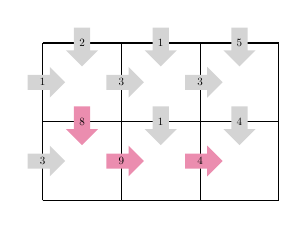
\begin{tikzpicture}
      \def\M{2}
      \def\N{3}
      \draw (0, 0) grid (\N,\M);

      \right{0}{1}{1}   \right{1}{1}{3}    \right{2}{1}{3}
      \right{0}{0}{3}   \right[h]{1}{0}{9} \right[h]{2}{0}{4}

      \down{0}{1}{2}    \down{1}{1}{1}     \down{2}{1}{5}
      \down[h]{0}{0}{8} \down{1}{0}{1}     \down{2}{0}{4}


      % \draw[->, >=latex, blue!20!white, line width=1cm] (0, 0) to node[black]{text} (5, 0);
    \end{tikzpicture}
  }
  \end{center}

  Las flechas marcadas de color {\color{red} rojo} representan un posible camino.
  Partiendo desde la casilla (1, 1) primero se mueve hacia la casilla (2, 1) obteniendo 8 puntos.
  Posteriormente se mueve dos veces a la derecha obteniendo respectivamente en cada movimiento
  9 y 4 puntos.
  El puntaje total es entonces $8 + 9 + 4 = 21$.
  Notar que cualquier otro camino obtiene un menor puntaje y por lo tanto 21 es el puntaje máximo
  que es posible obtener.

  Dada una matriz con los puntajes asociados a cada casilla, tu tarea es encontrar el puntaje máximo
  que es posible obtener en el juego.
\end{problemDescription}

\begin{inputDescription}
  La primera línea de la entrada contiene dos enteros $M$ y $N$ ($1 \leq N \leq 500$ y $1 \leq M \leq 500$)
  correspondientes respectivamente a la cantidad de filas y columnas en la matriz.

  A continuación siguen $M$ líneas cada una conteniendo $N$ enteros mayores o iguales que cero y menores
  que $10^6$.
  El $j$-ésimo entero de la línea $i$-ésima corresponde al puntaje asociado a moverse {\bf desde arriba}
  a la casilla $(i, j)$.

  Finalmente, vienen $M$ líneas más cada una conteniendo $N$ enteros mayores o iguales que cero.
  El $j$-ésimo entero de la línea $i$-ésima corresponde al puntaje asociado a moverse {\bf desde la izquierda}
  a la casilla $(i, j)$.
\end{inputDescription}

\begin{outputDescription}
\end{outputDescription}

\begin{scoreDescription}
  \subtask{10}
  Se probarán varios casos en que $M=1$ (ver primer caso de ejemplo).
  \subtask{10}
  Se probarán varios casos en que el puntaje asociado a moverse desde arriba es igual al puntaje
  de moverse desde la izquierda y además este es igual para todas las celdas
  (ver segundo caso de ejemplo).
  \subtask{30}
  Se probarán varios casos en que para cada celda el puntaje de moverse desde arriba es igual al
  puntaje de moverse desde la izquierda. Este valor puede ser distinto para celdas distintas
  (ver tercer caso de ejemplo).
  \subtask{50}
  Se probarán varios casos sin restricciones adicionales
  (ver cuarto caso de ejemplo).
\end{scoreDescription}

\begin{sampleDescription}
\sampleIO{sample-1}
\sampleIO{sample-2}
\sampleIO{sample-3}
\sampleIO{sample-4}
\end{sampleDescription}

\end{document}
